\documentclass[
	ngerman,
	toc=listof, % Abbildungsverzeichnis sowie Tabellenverzeichnis in das Inhaltsverzeichnis aufnehmen
	toc=bibliography, % Literaturverzeichnis in das Inhaltsverzeichnis aufnehmen
	footnotes=multiple, % Trennen von direkt aufeinander folgenden Fußnoten
	parskip=half, % vertikalen Abstand zwischen Absätzen verwenden anstatt horizontale Einrückung von Folgeabsätzen
	numbers=noendperiod % Den letzten Punkt nach einer Nummerierung entfernen (nach DIN 5008)
]{scrartcl}
\pdfminorversion=5 % erlaubt das Einfügen von pdf-Dateien bis Version 1.7, ohne eine Fehlermeldung zu werfen (keine Garantie für fehlerfreies Einbetten!)

% Dokumenteninformationen ----------------------------------------------------
\newcommand{\titel}{Anforderungsanalyse}
\newcommand{\untertitel}{Studienarbeit \semester}
\newcommand{\kompletterTitel}{\titel{} \\ \untertitel}
\newcommand{\datum}{\today}

\newcommand{\vorlagenOrdner}{../../99_Vorlagen} % Falls im Unterordner ../ vorne hinzufügen

\newcommand{\betriebLogo}{\vorlagenOrdner/Bilder/logo}

% Konfiguration -------------------------------------------------------------
\newcommand{\autoren}{
    \author{
        Schmid, Mike\\
        \texttt{sgschwin@hsr.ch}
        \and
        Schlatter, Janik\\
        \texttt{jschlatt@hsr.ch}
    }
}

\newcommand{\betreuer}{
    Stettler Beat\\
    \scriptsize \texttt{\url{beat.stettler@hsr.ch}}
    \normalsize
}

\newcommand{\schmid}{
    Mike Schmid\\
    \url{mschmid@hsr.ch}
    \normalsize
}

\newcommand{\schlatter}{
    Janik Schlatter\\
    \scriptsize \url{jschlatt@hsr.ch}
    \normalsize
}

\newcommand{\autorenNamen}{
    M. Schmid, J. Schlatter
}

\newcommand{\semester}{FS-2020}
\newcommand{\betriebName}{\textsc{HSR} Hochschule für Technik Rapperswil} % Metadaten zu diesem Dokument (Autor usw.)
% !TEX root = ../Projektdokumentation.tex

% Anpassung an Landessprache ---------------------------------------------------
\usepackage[english, main=ngerman]{babel} % \selectlanguage{english} if  needed

% Umlaute ----------------------------------------------------------------------
%   Umlaute/Sonderzeichen wie äüöß direkt im Quelltext verwenden (CodePage).
%   Erlaubt automatische Trennung von Worten mit Umlauten.
% ------------------------------------------------------------------------------
\usepackage[T1]{fontenc}
\usepackage[utf8]{inputenc}
\usepackage{textcomp} % Euro-Zeichen etc.

% Schrift ----------------------------------------------------------------------
\usepackage{lmodern} % bessere Fonts
\usepackage{relsize} % Schriftgröße relativ festlegen

% Tabellen ---------------------------------------------------------------------
\PassOptionsToPackage{table}{xcolor}
\usepackage{tabularx}
\usepackage{tabulary}
\usepackage{booktabs}
\usepackage{makecell}
\usepackage[table,xcdraw]{xcolor}
% für lange Tabellen
\usepackage{longtable}
\usepackage{array}
\usepackage{ragged2e}
\usepackage{lscape}
% Multi Columns
\usepackage{multicol}

% Grafiken ---------------------------------------------------------------------
\usepackage[dvips,final]{graphicx} % Einbinden von JPG-Grafiken ermöglichen
\usepackage{graphics} % keepaspectratio
\usepackage{floatflt} % zum Umfließen von Bildern
\graphicspath{{Bilder/}} % hier liegen die Bilder des Dokuments

% Sonstiges --------------------------------------------------------------------
\usepackage[titles]{tocloft} % Inhaltsverzeichnis DIN 5008 gerecht einrücken
\usepackage{enumitem} % anpassbare Enumerates/Itemizes
\usepackage{xspace} % sorgt dafür, dass Leerzeichen hinter parameterlosen Makros nicht als Makroendezeichen interpretiert werden

\usepackage{makeidx} % für Index-Ausgabe mit \printindex
\usepackage[printonlyused]{acronym} % es werden nur benutzte Definitionen aufgelistet

% Einfache Definition der Zeilenabstände und Seitenränder etc.
\usepackage{setspace}
\usepackage{geometry}

% Symbolverzeichnis
\usepackage[intoc]{nomencl}
\let\abbrev\nomenclature
\renewcommand{\nomname}{Abkürzungsverzeichnis}
\setlength{\nomlabelwidth}{.25\hsize}
\renewcommand{\nomlabel}[1]{#1 \dotfill}
\setlength{\nomitemsep}{-\parsep}

\usepackage{varioref} % Elegantere Verweise. „auf der nächsten Seite“
\usepackage{url} % URL verlinken, lange URLs umbrechen etc.

\usepackage{chngcntr} % fortlaufendes Durchnummerieren der Fußnoten
% \usepackage[perpage]{footmisc} % Alternative: Nummerierung der Fußnoten auf jeder Seite neu

\usepackage{ifthen} % bei der Definition eigener Befehle benötigt
\usepackage{todonotes} % definiert u.a. die Befehle \todo und \listoftodos
\usepackage[square]{natbib} % wichtig für korrekte Zitierweise

% PDF-Optionen -----------------------------------------------------------------
\usepackage{pdfpages}
\pdfminorversion=5 % erlaubt das Einfügen von pdf-Dateien bis Version 1.7, ohne eine Fehlermeldung zu werfen (keine Garantie für fehlerfreies Einbetten!)
\usepackage[
    bookmarks,
    bookmarksnumbered,
    bookmarksopen=true,
    bookmarksopenlevel=1,
    colorlinks=true,
% diese Farbdefinitionen zeichnen Links im PDF farblich aus
    linkcolor=AOBlau, % einfache interne Verknüpfungen
    anchorcolor=AOBlau,% Ankertext
    citecolor=AOBlau, % Verweise auf Literaturverzeichniseinträge im Text
    filecolor=AOBlau, % Verknüpfungen, die lokale Dateien öffnen
    menucolor=AOBlau, % Acrobat-Menüpunkte
    urlcolor=AOBlau,
% diese Farbdefinitionen sollten für den Druck verwendet werden (alles schwarz)
    %linkcolor=black, % einfache interne Verknüpfungen
    %anchorcolor=black, % Ankertext
    %citecolor=black, % Verweise auf Literaturverzeichniseinträge im Text
    %filecolor=black, % Verknüpfungen, die lokale Dateien öffnen
    %menucolor=black, % Acrobat-Menüpunkte
    %urlcolor=black,
%
    %backref, % Quellen werden zurück auf ihre Zitate verlinkt
    pdftex,
    plainpages=false, % zur korrekten Erstellung der Bookmarks
    pdfpagelabels=true, % zur korrekten Erstellung der Bookmarks
    hypertexnames=false, % zur korrekten Erstellung der Bookmarks
    linktocpage % Seitenzahlen anstatt Text im Inhaltsverzeichnis verlinken
]{hyperref}
% Befehle, die Umlaute ausgeben, führen zu Fehlern, wenn sie hyperref als Optionen übergeben werden
\hypersetup{
    pdftitle={\titel -- \untertitel},
    pdfauthor={\autoren},
    pdfcreator={\autoren},
    pdfsubject={\titel -- \untertitel},
    pdfkeywords={\titel -- \untertitel},
}


% zum Einbinden von Programmcode -----------------------------------------------
\usepackage{listings}
\usepackage{xcolor}
\usepackage{beramono}
% Pseudocode
\usepackage{algorithmic}
\usepackage[linesnumbered,ruled]{algorithm2e}

\definecolor{hellgelb}{rgb}{1,1,0.9}
\definecolor{colKeys}{rgb}{0,0,1}
\definecolor{colIdentifier}{rgb}{0,0,0}
\definecolor{colComments}{rgb}{0,0.5,0}
\definecolor{colString}{rgb}{1,0,0}
\definecolor{bluekeywords}{rgb}{0,0,1}
\definecolor{greencomments}{rgb}{0,0.5,0}
\definecolor{redstrings}{rgb}{0.64,0.08,0.08}
\definecolor{xmlcomments}{rgb}{0.5,0.5,0.5}
\definecolor{types}{rgb}{0.17,0.57,0.68}
\definecolor{DarkPurple}{rgb}{0.4, 0.1, 0.4}
\definecolor{DarkCyan}{rgb}{0.0, 0.5, 0.4}
\definecolor{LightLime}{rgb}{0.3, 0.5, 0.4}
\definecolor{Blue}{rgb}{0.0, 0.0, 1.0}
\definecolor{AOBlau}{rgb}{0, 0.28, 0.56}
% Tabellenfärbung:
\definecolor{heading}{rgb}{0.64,0.78,0.86}
\definecolor{odd}{rgb}{0.9,0.9,0.9}

\lstset{
    float=hbp,
	basicstyle=\footnotesize,
    identifierstyle=\color{colIdentifier},
    keywordstyle=\color{colKeys},
    stringstyle=\color{colString},
    commentstyle=\color{colComments},
    backgroundcolor=\color{hellgelb},
    columns=flexible,
    tabsize=2,
    frame=single,
    extendedchars=true,
    showspaces=false,
    showstringspaces=false,
    numbers=left,
    numberstyle=\tiny,
    breaklines=true,
    breakautoindent=true,
	captionpos=b,
}
\lstdefinestyle{visual-studio-style}{
	language=[Sharp]C,
	columns=flexible,
	showstringspaces=false,
	basicstyle=\footnotesize\ttfamily, 
	commentstyle=\color{greencomments},
	morekeywords={partial, var, value, get, set},
	keywordstyle=\bfseries\color{bluekeywords},
	stringstyle=\color{redstrings},
	breaklines=true,
	breakatwhitespace=true,
	tabsize=4,
	numbers=left,
	numberstyle=\tiny\color{black},
	frame=lines,
	showspaces=false,
	showtabs=false,
	escapeinside={£}{£},
}
\lstdefinestyle{eclipse-style}{
	language=Java,  
	columns=flexible,
	showstringspaces=false,     
	basicstyle=\footnotesize\ttfamily, 
	keywordstyle=\bfseries\color{DarkPurple},
	commentstyle=\color{LightLime},
	stringstyle=\color{Blue}, 
	escapeinside={£}{£}, % latex scope within code      
	breaklines=true,
	breakatwhitespace=true,
	showspaces=false,
	showtabs=false,
	tabsize=4,
	morekeywords={length},
	numbers=left,
	numberstyle=\tiny\color{black},
	frame=lines,
}
\lstset{style=eclipse-style}
\lstdefinelanguage{cs}{
	sensitive=false,
	morecomment=[l]{//},
	morecomment=[s]{/*}{*/},
	morestring=[b]",
	morekeywords={
		abstract,event,new,struct,as,explicit,null,switch
		base,extern,object,this,bool,false,operator,throw,
		break,finally,out,true,byte,fixed,override,try,
		case,float,params,typeof,catch,for,private,uint,
		char,foreach,protected,ulong,checked,goto,public,unchecked,
		class,if,readonly,unsafe,const,implicit,ref,ushort,
		continue,in,return,using,decimal,int,sbyte,virtual,
		default,interface,sealed,volatile,delegate,internal,short,void,
		do,is,sizeof,while,double,lock,stackalloc,
		else,long,static,enum,namespace,string},
}
\lstdefinelanguage{natural}{
	sensitive=false,
	morecomment=[l]{/*},
	morestring=[b]",
	morestring=[b]',
	alsodigit={-,*},
	morekeywords={
		DEFINE,DATA,LOCAL,END-DEFINE,WRITE,CALLNAT,PARAMETER,USING,
		IF,NOT,END-IF,ON,*ERROR-NR,ERROR,END-ERROR,ESCAPE,ROUTINE,
		PERFORM,SUBROUTINE,END-SUBROUTINE,CONST,END-FOR,END,FOR,RESIZE,
		ARRAY,TO,BY,VALUE,RESET,COMPRESS,INTO,EQ},
}
\lstdefinelanguage{php}{
	sensitive=false,
	morecomment=[l]{/*},
	morestring=[b]",
	morestring=[b]',
	alsodigit={-,*},
	morekeywords={
		abstract,and,array,as,break,case,catch,cfunction,class,clone,const,
		continue,declare,default,do,else,elseif,enddeclare,endfor,endforeach,
		endif,endswitch,endwhile,extends,final,for,foreach,function,global,
		goto,if,implements,interface,instanceof,namespace,new,old_function,or,
		private,protected,public,static,switch,throw,try,use,var,while,xor
		die,echo,empty,exit,eval,include,include_once,isset,list,require,
		require_once,return,print,unset},
}
 % verwendete Packages
% !TEX root = ../Projektdokumentation.tex

% Seitenränder -----------------------------------------------------------------
\setlength{\topskip}{\ht\strutbox} % behebt Warnung von geometry
\geometry{
	a4paper,
	left=20mm,
	right=20mm,
	top=25mm,
	bottom=40mm
}

\usepackage[
	automark, % Kapitelangaben in Kopfzeile automatisch erstellen
	headsepline, % Trennlinie unter Kopfzeile
	% footsepline, % Trennlinie oberhalb Fusszeile
	ilines % Trennlinie linksbündig ausrichten
]{scrpage2}

% Kopf- und Fußzeilen ----------------------------------------------------------
\pagestyle{scrheadings}
% chapterpagestyle gibt es nicht in scrartcl
%\renewcommand{\chapterpagestyle}{scrheadings}
\clearscrheadfoot

% Kopfzeile
\renewcommand{\headfont}{\normalfont} % Schriftform der Kopfzeile
\ihead{\large{\textsc{\titel}}\\ \small{\untertitel} \\[2ex] \textit{\headmark}}
\chead{}
%\ohead{\includegraphics[scale=0.125]{\betriebLogo}}
\setlength{\headheight}{20mm} % Höhe der Kopfzeile
%\setheadwidth[0pt]{textwithmarginpar} % Kopfzeile über den Text hinaus verbreitern (falls Logo den Text überdeckt)

% Fußzeile
\ifoot{\autorenNamen}
\cfoot{}
\ofoot{\pagemark}

% Überschriften nach DIN 5008 in einer Fluchtlinie
% ------------------------------------------------------------------------------

% Abstand zwischen Nummerierung und Überschrift definieren
% > Schön wäre hier die dynamische Berechnung des Abstandes in Abhängigkeit
% > der Verschachtelungstiefe des Inhaltsverzeichnisses
\newcommand{\headingSpace}{1.5cm}

% Abschnittsüberschriften im selben Stil wie beim Inhaltsverzeichnis einrücken
\renewcommand*{\othersectionlevelsformat}[3]{
  \makebox[\headingSpace][l]{#3\autodot}
}

% Für die Einrückung wird das Paket tocloft benötigt
%\cftsetindents{chapter}{0.0cm}{\headingSpace}
\cftsetindents{section}{0.0cm}{\headingSpace}
\cftsetindents{subsection}{0.0cm}{\headingSpace}
\cftsetindents{subsubsection}{0.0cm}{\headingSpace}
\cftsetindents{figure}{0.0cm}{\headingSpace}
\cftsetindents{table}{0.0cm}{\headingSpace}

% Allgemeines
% ------------------------------------------------------------------------------

\onehalfspacing % Zeilenabstand 1,5 Zeilen
\frenchspacing % erzeugt ein wenig mehr Platz hinter einem Punkt

% Schusterjungen und Hurenkinder vermeiden
\clubpenalty = 10000
\widowpenalty = 10000
\displaywidowpenalty = 10000

% Quellcode-Ausgabe formatieren
\lstset{numbers=left, numberstyle=\tiny, numbersep=5pt, breaklines=true}
\lstset{emph={square}, emphstyle=\color{red}, emph={[2]root,base}, emphstyle={[2]\color{blue}}}

\counterwithout{footnote}{section} % Fußnoten fortlaufend durchnummerieren
\setcounter{tocdepth}{\subsubsectionlevel} % im Inhaltsverzeichnis werden die Kapitel bis zum Level der subsubsection übernommen
\setcounter{secnumdepth}{\subsubsectionlevel} % Kapitel bis zum Level der subsubsection werden nummeriert

% Aufzählungen anpassen
\renewcommand{\labelenumi}{\arabic{enumi}.}
\renewcommand{\labelenumii}{\arabic{enumi}.\arabic{enumii}.}
\renewcommand{\labelenumiii}{\arabic{enumi}.\arabic{enumii}.\arabic{enumiii}}
 % Definitionen zum Aussehen der Seiten
% !TEX root = ../Projektdokumentation.tex

% Abkürzungen, ggfs. mit korrektem Leerraum
\newcommand{\bs}{$\backslash$\xspace}
\newcommand{\bspw}{bspw.\xspace}
\newcommand{\bzw}{bzw.\xspace}
\newcommand{\ca}{ca.\xspace}
\newcommand{\dahe}{\mbox{d.\,h.}\xspace}
\newcommand{\etc}{etc.\xspace}
\newcommand{\eur}[1]{\mbox{#1\,\texteuro}\xspace}
\newcommand{\evtl}{evtl.\xspace}
\newcommand{\ggfs}{ggfs.\xspace}
\newcommand{\Ggfs}{Ggfs.\xspace}
\newcommand{\gqq}[1]{\glqq{}#1\grqq{}}
\newcommand{\inkl}{inkl.\xspace}
\newcommand{\insb}{insb.\xspace}
\newcommand{\ua}{\mbox{u.\,a.}\xspace}
\newcommand{\usw}{usw.\xspace}
\newcommand{\Vgl}{Vgl.\xspace}
\newcommand{\zB}{\mbox{z.\,B.}\xspace}

% Befehle für häufig anfallende Aufgaben
\newcommand{\Abbildung}[1]{\autoref{fig:#1}}
\newcommand{\Anhang}[1]{\appendixname{}~\ref{#1}: \nameref{#1} \vpageref{#1}}
\newcommand{\includegraphicsKeepAspectRatio}[2]{\includegraphics[width=#2\textwidth,height=#2\textheight,keepaspectratio]{#1}}
\newcommand{\Zitat}[2][\empty]{\ifthenelse{\equal{#1}{\empty}}{\citep{#2}}{\citep[#1]{#2}}}
\newcommand{\Autor}[1]{\textsc{#1}} % zum Ausgeben von Autoren
\newcommand{\itemd}[2]{\item{\textbf{#1}}\\{#2}} % erzeugt ein Listenelement mit fetter Überschrift

% einfaches Wechseln der Schrift, z.B.: \changefont{cmss}{sbc}{n}
\newcommand{\changefont}[3]{\fontfamily{#1} \fontseries{#2} \fontshape{#3} \selectfont}

% Verwendung analog zu \includegraphics
\newlength{\myx} % Variable zum Speichern der Bildbreite
\newlength{\myy} % Variable zum Speichern der Bildhöhe
\newcommand\includegraphicstotab[2][\relax]{%
% Abspeichern der Bildabmessungen
\settowidth{\myx}{\includegraphics[{#1}]{#2}}%
\settoheight{\myy}{\includegraphics[{#1}]{#2}}%
% das eigentliche Einfügen
\parbox[c][1.1\myy][c]{\myx}{%
\includegraphics[{#1}]{#2}}%
}

% verschiedene Befehle um Wörter semantisch auszuzeichnen ----------------------
\newcommand{\Index}[2][\empty]{\ifthenelse{\equal{#1}{\empty}}{\index{#2}#2}{\index{#1}#2}}
\newcommand{\Fachbegriff}[2][\empty]{\ifthenelse{\equal{#1}{\empty}}{\textit{\Index{#2}}}{\textit{\Index[#1]{#2}}}}
\newcommand{\NeuerBegriff}[2][\empty]{\ifthenelse{\equal{#1}{\empty}}{\textbf{\Index{#2}}}{\textbf{\Index[#1]{#2}}}}

\newcommand{\Ausgabe}[1]{\texttt{#1}}
\newcommand{\Eingabe}[1]{\texttt{#1}}
\newcommand{\Code}[1]{\texttt{#1}}
\newcommand{\Datei}[1]{\texttt{#1}}

\newcommand{\Assembly}[1]{\textsf{#1}}
\newcommand{\Klasse}[1]{\textsf{#1}}
\newcommand{\Methode}[1]{\textsf{#1}}
\newcommand{\Attribut}[1]{\textsf{#1}}

\newcommand{\Datentyp}[1]{\textsf{#1}}
\newcommand{\XMLElement}[1]{\textsf{#1}}
\newcommand{\Webservice}[1]{\textsf{#1}}

\newcommand{\Refactoring}[1]{\Fachbegriff{#1}}
\newcommand{\CodeSmell}[1]{\Fachbegriff{#1}}
\newcommand{\Metrik}[1]{\Fachbegriff{#1}}
\newcommand{\DesignPattern}[1]{\Fachbegriff{#1}}

\newcommand{\muss}[1]{\textcolor{red}{#1}}
\newcommand{\soll}[1]{\textcolor{orange}{#1}}
\newcommand{\kann}[1]{\textcolor{blue}{#1}}

\newcommand{\success}[1]{\textcolor{greencomments}{#1}}
\newcommand{\fail}[1]{\textcolor{red}{#1}} % eigene allgemeine Befehle, die z.B. die Arbeit mit LaTeX erleichtern

\begin{document}

% Deckblatt ------------------------------------------------------------------
\phantomsection
\thispagestyle{plain}
\pdfbookmark[1]{Deckblatt}{deckblatt}
\begin{titlepage}
    \begin{center}
        \includegraphics[scale=1.5]{\betriebLogo}\\[10ex]

        \rule{\linewidth}{0.5mm}\\[2ex]
        {\huge \bfseries  \titel }\\[2ex]
        {\LARGE \untertitel }\\[2ex]
        {\large \datum}\\
        \rule{\linewidth}{0.5mm}\\[10ex]

        \begin{minipage}[t]{0.4\textwidth}
            \begin{flushleft} 
                \large \emph{Autoren:}\\
                    \large Mike \textsc{Schmid}\\
                    \scriptsize \texttt{mike.schmid@hsr.ch}\\[1ex]
                    \large Janik \textsc{Schlatter}\\
                    \scriptsize \texttt{janik.schlatter@hsr.ch}\\[1ex]
            \end{flushleft}
            \end{minipage}
            ~
            \begin{minipage}[t]{0.4\textwidth}
            \begin{flushright} 
                \large \emph{Supervisor:} \\
                Prof. Stettler \textsc{Beat}\\
                \scriptsize \texttt{beat.stettler@hsr.ch}\\[1ex]
            \end{flushright}
        \end{minipage}\\[40ex]

        \small
        \noindent
        Dieses Werk einschließlich seiner Teile ist \textbf{urheberrechtlich geschützt}.
        Jede Verwertung außerhalb der engen Grenzen des Urheberrechtgesetzes ist ohne
        Zustimmung des Autors unzulässig und strafbar. Das gilt insbesondere für
        Vervielfältigungen, Übersetzungen, Mikroverfilmungen sowie die Einspeicherung
        und Verarbeitung in elektronischen Systemen.

    \end{center}
\end{titlepage}
\cleardoublepage

% Preface --------------------------------------------------------------------
\pagenumbering{Roman}

\section{Sinn und Zweck}
Dieses Dokument beschreibt die Anforderungen an die Studienarbeit Nuts 2.0.
Es umfasst eine Übersicht über die Problemdomäne, die Requirements-Analyse und die nichtfunktionalen Anforderungen an das zu entwickelnde System.

% Änderungsgeschichte
\section*{Änderungsgeschichte}
\begin{tabularx}{\textwidth}{llXl}
	\toprule
	Datum & Version & Änderung & Autor \\
	\midrule
	03.03.2020 & 1.0 & Initial Setup & Janik Schlatter \\
	11.03.2020 & 1.0 & Fertigstellung für Meilenstein: Requirements & Janik Schlatter, Mike Schmid \\
	12.03.2020 & 2.0 & Revision gem. Beschprechung vom 11.03.2020 & Janik Schlatter, Mike Schmid \\
	\bottomrule
\end{tabularx}
\cleardoublepage

% Inhaltsverzeichnis
\phantomsection
\pdfbookmark[1]{Inhaltsverzeichnis}{inhalt}
\tableofcontents
\cleardoublepage

\pagenumbering{arabic}
% Jede Überschrift 1 auf neuer Seite
\let\stdsection\section
\renewcommand\section{\clearpage\stdsection}

% Inhalt ---------------------------------------------------------------------
\section{Übersicht Problemstellung}
	\subsection{Generell}
		Bei der Entwicklung von Netzwerkumgebungen werden auch in modernen Systemen die Überprüfungen und Tests der Konfigurationen meistens von Hand vorgenommen.
		Die Applikation soll ein Framework zur Verfügung stellen, mit dem Netzwerke automatisiert getestet werden können, vergleichbar mit Unit-Tests in der Software-Entwicklung.
		Die folgenden Abschnitte sollen aufzeigen, welche Herausforderungen an ein solches System gestellt werden und wie ein Framework damit umgehen könnte.
		Dazu wurden die Kern-Akteure in einem Netzwerk identifiziert und deren Funktionalität und gegenseitige Abhängigkeiten so generalisiert wie möglich formuliert, um auf dieser Basis die Testsoftware zu entwerfen.
		Es wurden Annahmen bezüglich der Namensgebung getroffen. Beispielsweise sind die Bezeichnungen der einzelnen Netzwerk-Techniker überall ein wenig anders formuliert.
		\newpage

	\subsection{Akteure im aktuellen System}
	\label{sec:Akteure}
	Die hier beschriebenen Akteure sind in einem herkömmlichen Netzwerksystem anzutreffen. 
	
	\begin{table}[!h]
		\begin{tabularx}{\textwidth}{lX}
			\toprule
			Akteur &  Beschreibung \\
			\midrule
			Netzwerk-Architekt  & Ein Netzwerk-Architekt plant und erstellt Kommunikationsnetzwerke. 
			In der Praxis oft auch als Network-Engineer bezeichnet. 
			Im Zuge dieser Arbeit wurde zwischen dem Architekten als Verantwortlichen Senior Network Engineer und einem Network Engineer (Junior oder Senior) als operativen Mitarbeiter unterschieden. 
			Der Architekt nimmt dabei eher die Rolle des Managers oder Teamleiters ein. Er führt dabei normalerweise keine Konfigurationen am Netzwerk durch. \\ 
			Netzwerk-Engineer  & Ein Netzwerk-Engineer ist für die Installation und Instandhaltung eines Netzwerks zuständig. 
			Er ist dem Netzwerk-Architekten unterstellt und setzt mit Ihm zusammen die geplanten Arbeiten um. \\
			Netzwerk-Administrator  & Der Netzwerk Administrator hat üblicherweise eine abgeschlossene Berufslehre in der Informatik und arbeitet zusammen mit dem Netzwerk-Engineer am Netzwerk. 
			Es wird davon ausgegangen, dass ein Netz-Admin wenige bis keine Programmierkenntnisse hat. 
			Ein Netzwerk Administrator hat, je nach Grösse des Netzwerks, nur Kenntnisse über einen Teil der Netzwerkumgebung. 
			Er führt dabei ihm vom Architekten oder Engineer vorgegebene Arbeiten aus und muss dazu nicht den vollen Überblick über das Netzwerk und die darin verwendeten Technologien kennen.\\
			Netzwerk-User & Benutzer der Netzwerkumgebung. User müssen das Netzwerk verwenden, aber nicht dessen Konfigurationen anpassen können. \\
			\midrule
			Netzwerk-Gerät  & Ein Netzwerkgerät kann aus Hardware wie Switch, Router oder Server bestehen oder Virtuell als Software implementiert sein. Im Zuge der Arbeit werden Netzwerkgeräte auch als Netzwerk-Devices oder einfach Device bezeichnet. Typischerweise haben Devices eine Statische Konfiguration und einen Zustand zur Laufzeit. In den kommenden Kapiteln wird genauer auf Netzwerkgeräte eingegangen. \\
			Repository/Inventar &  Im Inventar werden die Unterschiedlichen Devices mit den für den Betrieb wichtigsten Parametern abgelegt. Das Inventar kann in digitaler Form als Repository, als File auf einem Ordner/Computer, oder analog in einem Order abgelegt sein. Das Inventar wird benötigt, um die aktuellen Konfigurationen, die physische Position des Geräts oder sonstige für den Betrieb relevanten Informationen zu dokumentieren. \\
			\bottomrule
		\end{tabularx}
			\caption{Akteure in einem Netzwerksystem}
	\end{table}
	
	\newpage

	\subsection{Zusätzliche Entitäten im zu entwickelnden System}
	Diese Entitäten müssen zusätzlich zu den im Abschnitt \ref{sec:Akteure} beschriebenen Akteuren in einem Netzwerk, welches ein System für das automatisierte Testen beinhaltet, auftreten.
	
	\begin{table}[!h]
		\begin{tabularx}{\textwidth}{lX}
			\toprule
			Testprogramm &  Das Testprogramm ist das zu entwickelnde System in dieser Arbeit. Es interagiert mit den anderen Akteuren und hat, abhängig von Akteur und Kontext, unterschiedliche Anforderungen. \\
			Testdefinitionssprache & Kann auch Testbeschreibungssprache genannt werden. Testbeschreibungen sollten zwischen dem Systemmodell und den low-level-Testcases angelegt werden und möglichst einfach und allgemein aufgebaut sein. Eine Testdefinition beschreibt unabhängig von der zu verwendeten Programmiersprache oder ausführenden Plattform die einzelnen Testfälle. \\
			Testreport & Ausgabewerte der durchgeführten Tests. Reports sollten so strukturiert sein, dass ein Netzwerk-Techniker mit wenig Aufwand erkennen kann, welche Tests erfolgreich verlaufen sind, welche nicht erfolgreich waren und was mögliche Ursachen dafür waren. Testreports können in der Dokumentenablage des ausführenden Systems oder in einem Repository abgelegt werden und benötigen neben den Testfällen im Minimum noch ein Durchführungsdatum und -Uhrzeit. \\
			\midrule
			Kommunikationskanal & Der Kommunikationskanal verbindet das zu testende Netzwerk mit dem Testprogramm. Abhängig vom Netzwerk geschieht dies über Kabelverbindungen oder Kabellos. Es gibt verschiedene Technologien, die die Kommunikation über das Medium ermöglichen und je nach Schnittstelle unterschiedliche Ergebnisse und -formate liefert. \\
			Netzwerktest & Werden meistens von Hand oder über Scripts ausgeführt. Ein automatisierter Netzwerktest sollte hypothetisch ad-hoc nach jeder Konfigurationsänderung durchgeführt werden um zu validieren, dass das Netzwerk noch wie gewollt läuft. \\
			\bottomrule
		\end{tabularx}
		\caption{Entitäten im zu entwickelnden System}
	\end{table}
	\newpage

	\subsection{Herausforderungen}
	Das Testen von Netzwerken ist ein komplexes Unterfangen. 
	Der Netzwerkzustand ändert sich zur Laufzeit dauernd, um sich an Änderungen von einzelnen Geräten anzupassen.
	User treten dem Netzwerk bei oder verlassen dieses und Netzwerkgeräte passen über dynamische Protokolle die Verbindungen an um eine möglichst performante Verbindung zu ermöglichen oder um Fehler/Ausfälle zu korrigieren.
	Weiterhin können spezielle Konfigurationen wie die Priorisierung von verschiedenen Kommunikationsarten z.B. Internettelefonie (VoIP), auch Quality of Service (QoS) genannt, im System vorkommen, was die genaue Erfassung des Ist-Zustandes noch komplizierter macht.
	In diesem Kontext muss ein Netzwerk-Testsystem nicht nur die Gerätekonfiguration beim Starten, sondern auch die dynamische Laufzeitkonfiguration berücksichtigen.
	
	\subsection{Beschreibung Software-Unit-Testing}
	Das Testen von Software kann grob in zwei Kategorien unterteilt werden, statisch und dynamisch. 
	Darüber hinaus gibt es weitere Unterteilungen, je nachdem, was in welchem Umfang wie getestet werden soll. Die Unittests sind dabei in der dynamischen Kategorie angesiedelt und dienen der Verifikation der Software-Implementation.

	Statische Tests umfassen Code- und Design-Review, Code-Guidelines und formale Methoden.

	Dynamische Tests sind üblicherweise Softwarebestandteile, die andere Komponenten mit verschiedenen Methoden auf die korrekte Ausführung testen. 

		\subsubsection{Anforderungen an Softwaretests}
		Softwaretests müssen folgende Anforderungen erfüllen:

		Die Tests müssen geplant sein und es muss ein Test Plan existieren.

		Tests müssen systematisch spezifiziert sein.

		Die Resultate der Tests müssen dokumentiert werden.

		Nach Möglichkeit sollen Tests automatisch ausgeführt werden.

		Tests müssen reproduzierbar und nachvollziehbar sein, d.H. sie müssen sich im Debugger Schritt für Schritt durchführen lassen.
			
\section{Detailbeschreibung Akteure}
Dieser Abschnitt beschreibt die Akteure, welche im Abschnitt \ref{sec:Akteure} genannt werden und ihre spezifischen Anforderungen an ein Testsystem sowie Einschränkungen, die vom System auf die Akteure gelten.
	
	\subsection{Personen}
	Akteure interagieren mit dem zu entwickelnden System und hat in dessen Kontext eine Rolle und Ziele.
	Akteure lassen sich in drei Kategorien unterteilen: 
		
	\begin{table}[!h]
		\begin{tabularx}{\textwidth}{lX}
			\toprule
				Primärer Aktor & Person oder Objekt, dessen ziele durch Interaktion mit dem zu entwickelnden System erfüllt werden.\\
				Unterstützender Akteur & Bietet dem System Services an, z.B. Techniksupport eines Herstellers.\\
				Nebenaktor & Hat Interesse am Verhalten des Systems oder zieht einen Nutzen daraus, ist aber nicht primär oder unterstützend. \\
			\bottomrule
		\end{tabularx}
		\caption{Kategorien der Akteure}
	\end{table}

		\subsubsection{Netzwerk-Architekt}
		
			\paragraph{Rolle} ~\\
			Primärer Aktor 

			\paragraph{Ziele} ~\\ 
			Konfiguration automatisierter Tests (welche er für analytische Zwecke benötigt) 
			Durchführung der Tests, 
			Sichten der Resultate
			
		\subsubsection{Netzwerk-Engineer}
		
			\paragraph{Rolle} ~\\
			Primärer Aktor 

			\paragraph{Ziele} ~\\
			Verwalten von Devices in einem Inventar, 
			Konfiguration automatisierter Tests, 
			Durchführung der Tests, 
			Sichten der Resultate
			Erweiterung des Testsystems
			\newpage

		\subsubsection{Netzwerk-Administrator}

			\paragraph{Rolle} ~\\
			Primärer Aktor 
			\paragraph{Ziele} ~\\
			Verwalten von Devices in einem Inventar, 
			Konfiguration automatisierter Tests (einfachere Tests, die für einen Administrator wichtig sind), 
			Durchführung der Tests, 
			Sichten der Resultate

		\subsubsection{User}

			\paragraph{Rolle} ~\\
			Nebenaktor 
			\paragraph{Ziele} ~\\
			Verwenden des Systems

		\subsubsection{Einschränkungen}

			\paragraph{Prioritärer Aktor} ~\\
			Das zu entwickelnde System wird primär mit dem Netzwerk-Engineer als Aktor aufgebaut, da der Architekt eher eine planende/managende Rolle einnimmt und der Administrator für einfachere Aufträge, wie das umschalten von Ports oder Interfaces, zusständig ist.


			\paragraph{User} ~\\
			Für das zu entwickelnde System hat der User keinen Einfluss auf die Funktionalen Anforderungen. 
			Er ist darauf angewiesen, dass das Netzwerk möglichst schnell und fehlerfrei funktioniert. 
			In den Nichtfunktionalen Anforderungen wird auf diese Bedürfnisse eingegangen.

			\paragraph{Kenntnisse der Netzwerk-Techniker} ~\\
			Um Tests auf dem Netzwerk effektiv durchführen zu können, benötigen die primären Akteure einige Fähigkeiten:

			Sie müssen wissen, wie sich das Netzwerk zur Laufzeit verhalten soll.

			Tester müssen Benutzeraktivitäten gegenüber dem Netzwerk imitieren können.

			Falls gewisse Devices nicht getestet werden können, müssen Tester deren Funktionalitäten bei Bedarf gegenüber dem Netzwerk imitieren können.

			Sie müssen wissen, was das Netzwerk als Reaktion auf ihre Aktivitäten macht.

			Tester müssen in der Lage sein, den Fortschritt und die Resultate der Tests zu interpretieren und die Ursachen von gescheiterten Tests ausfindig machen.


	\subsection{Devices}
	Um Tests durchführen zu können, werden mehrere Devices benötigt, die in einer bestehenden Konfiguration in einem Netzwerk integriert sind.
	Die Devices müssen dafür einen oder mehrere Kommunikationskanäle bereitstellen, über die man die Konfiguration abfragen und Befehle senden kann.
	Um einen Netzwerktest Schritt-für-Schritt durchführen zu können, werden verschiedene Zwischenschritte benötigt, welche die Anforderungen and das zu entwickelnde System darstellen.
	Geräte müssen mit ihrer Start-Konfiguration in einem Inventar erfasst werden, die Startkonfiguration und Laufzeitkonfiguration muss abrufbar und speicherbar sein,
	und die Geräte sollten sich in logische Gruppen, wie beispielsweise Aufteilung nach Gebäude oder nach VLAN (Virtual Local Area Network), kategorisieren lassen.

		\subsubsection{Devices erfassen}
			Das Erfassen von Geräten beinhaltet das Abrufen der Gerätekonfiguration und das Speichern dieser Konfiguration in einem Inventar. 
			Das Inventar kann mit einer Beschreibungssprache wie XML, YAML, YANG oder weitere, geführt werden, die es erlaubt, die Informationen dynamisch in das zu entwickelnden System zu laden und für die Testdefinition zu verwenden.
			Die Erfassung der Devices kann dabei in folgende Stufen unterteilt werden, die mit steigender Automatisierung ein komplexeres System voraussetzen.

			\begin{table}[!h]
				\begin{tabularx}{\textwidth}{lX}
					\toprule
					Stufe & Beschreibung\\
					\midrule
					Stufe Manuell & Die Devices werden vom Benutzer manuell in einem File hinzugefügt welches optimalerweise in einem Repository gespeichert wird. \\
					\midrule
					Stufe Formular & Der Netzwerk-Techniker kann mit Hilfe eines Formulars oder einem Grafikinterface des zu entwickelnden Systems die Devices erfassen. Da dies über ein Formular geschieht, muss der Benutzer nicht manuell für jedes Device ein neues File anlegen, sondern das Programm erledigt all das für den Benutzer und er kann sich das Inventar im GUI zusammenklicken.\\
					\midrule
					Stufe Automatisiert & Die Devices werden automatisch von dem zu entwickelnden System aus dem Netzwerk ausgelesen und in ein Inventar hinzugefügt. Das Ergebnis kann vom Techniker dann gesichtet werden und lässt sich bei Bedarf anpassen. \\
					\bottomrule
				\end{tabularx}
				\caption{Stufen der Device-Erfassung}
			\end{table}
			
			\newpage

		\subsubsection{Device Informationen}
			Je spezifischer die Tests des zu entwickelnden Programms sind, desto mehr Informationen eines einzelnen Devices werden benötigt.
			Die Informationen der Devices werden in Kategorien unterteilt: \textcolor{green}{Minimaleinstellungen} , \textcolor{yellow}{Erweiterte Einstellungen} und \textcolor{red}{Alle Informationen}.
			Je mehr Informationen von einem Gerät im Inventar abgelegt sind, desto mehr Tests lassen sich ohne Erfassung von zusätzlichen Infos durchführen. \\
			Die folgende Tabelle zählt einige Beispiele dieser Einstellungen auf und beschreibt, wozu die Informationen benötigt werden.

			\begin{table}[!h]
				\begin{tabularx}{\textwidth}{lX}
					\toprule
					Einstellung & Beschreibung\\
					\midrule
					\textcolor{green}{Name und Passwort} & Diese Informationen werden benötigt, um sich bei einem Device (z.B. Router) anzumelden, um dort Befehle für die Tests ausführen zu können. \\	
					\textcolor{green}{MAC-Adresse} & Die Media Access Control Adresse ist für die eindeutige Identifikation eines Netzwerkgerätes. Die MAC kann z.B. für die Berechnung von IPv6 Adressen verwendet werden.\\
					\textcolor{green}{IP Adresse} & Die IP-Adresse eines Devices ist die Virtuelle Adresse, die das Gerät im Netzwerk hat. \\
					\textcolor{green}{Seriennummer} & Die Seriennummer eines Geräts wird nur für sehr spezielle Anwendungen benötigt z.B. die Entscheidung des Wurzelknotens im Zweifelsfall beim Spanning Tree Protokoll. \\
					\midrule
					\textcolor{yellow}{Statische Routen} & Statische Routen sind manuell konfigurierte Einstellungen, die nicht verändert werden, wenn das Netz nicht angepasst wird. Sie sind einfach zu konfigurieren, aber sie können sich nicht an Systemfehler anpassen. \\
					\textcolor{yellow}{Dynamisches Routing} & Routing Protokolle passen die konfigurierten Routen der Geräte zur Laufzeit an, um auf Änderungen im Netz zu reagieren. Dynamische Protokolle sind flexibler, aber auch komplexer als statische Routen. \\
					\midrule
					\textcolor{red}{Virtual LAN} & Das Virtuelle Local Area Network unterteilt Geräte im Netzwerk in logische Gruppen und bewirkt eine Segmentierung des Netzwerks was zu erhöhter Sicherheit, Erweiterbarkeit und besserem Netzwerkmanagement führen kann. \\
					\textcolor{red}{Overlay Netzwerk} & In einem Overlay Netzwerk werden logische Verbindungen von der virtuellen Konfiguration getrennt. In jedem Layer nimmt ein physisches Gerät dabei eine andere Rolle wahr, was dazu führt, dass die Gerätekonfiguration schwieriger zu testen sind. \\				
					\bottomrule
				\end{tabularx}
				\caption{Beispiele für Device-Informationen}
			\end{table}
			
			\newpage

		\subsubsection{Device Gruppen}
			Die Devices sollen sich in logische Gruppen unterteilen lassen. Somit könnte man zum Beispiel alle Devices in einem Gebäude in die Gruppe: 'Gebäude 1' schieben.
			Im Kontext des zu entwickelnden Systems würde man damit die Möglichkeit haben, Filter auf die Geräte anzuwenden, um nur spezifische Einstellungen zu testen.

	\subsection{Netzwerktest}
		Netzwerktest werden von den Technikern in einer Testbeschreibungssprache erfasst und vom zu entwickelnden System automatisiert ausgeführt.
		Dabei werden verschiedene Anforderungen an eine Testbeschreibung gestellt. Zum Beispiel sollten sich Tests in logische Kategorien unterteilen lassen, die Erfassung der Tests soll möglichst automatisch durchführbar sein und die Ergebnisse der Tests müssen verständlich sein und sich in einem Report speichern lassen.

		
		\subsubsection{Test Kategorien/Typen}
			Die Tests werden grundsätzlich nach Kategorien unterschieden, beispielsweise sind alle Ping-Tests eine Art.
			Die Einteilung von Tests in Kategorien und Typen erlaubt es dem Tester, diese Tests im System zu filtern und Tests kategorisch auszuwählen, wenn er eine Testausführung plant.
			Ein wichtiger Anforderungspunkt ist dabei, dass Techniker in Zukunft möglichst einfach weitere Kategorien/Testarten hinzufügen können.

		\subsubsection{Test erfassen}
			Auch hier gibt es wieder mehrere Stufen, wie die Tests erfasst werden können.\\
			\begin{table}[!h]
				\begin{tabularx}{\textwidth}{lX}
					\toprule
					Stufe & Beschreibung\\
					\midrule
					Stufe Manuell & Der Benutzer erfasst die Tests komplett manuell in einem File mit einer Testdefinitionssprache. In diesem File muss der Benutzer die Testart, die beteiligten Devices und weitere Optionen des Testes festlegen. Ausserdem ist das zu erwartende Ergebnis für einen Test zu spezifizieren. \\
					\midrule
					Stufe Formular & Das Programm stellt ein Formular zur Verfügung, welches die ganze Testerfassung vereinfacht. Der Benutzer kann sich hierbei den Test nur noch über die Benutzeroberfläche zusammenklicken. Das Programm speichert danach den Test automatisch in einem File oder Repository. \\
					\bottomrule
				\end{tabularx}
				\caption{Stufen der Test-Erfassung}
			\end{table}
			

		\subsubsection{Erwartungswert erfassen}
			Ein Test findet in der Regel durch einen Vergleich vom Ist-Wert mit dem Soll-Wert statt. Der Ist-Wert in einem Netzwerk ist die Konfiguration und der Zustand zur Laufzeit. Der Sollwert muss vom Netzwerk-Techniker bei der Testdefinition erfasst werden.
			

		\subsubsection{Testreihenfolge}
			Es kann sein, dass vom Tester eine gewisse Reihenfolge für die Ausführung der Tests gewünscht ist. 
			Dafür sollten sich Tests nach Kategorie (Ping, Traceroute etc.), nach Layer, nach Gerätetyp (Switch, Router, Server, etc.) oder nach eigenen Kategorien (z.B. nur Gebäude 1), filtern lassen. 
			Die Auswahl der Testreihenfolge soll dabei möglichst intuitiv mit einer grafischen Benutzeroberfläche geschehen und mit wenigen Klicks durchführbar sein.

		\subsubsection{Test Durchführung}
			Wenn der Benutzer die Durchführung startet kann er mit Hilfe der Test-Gruppen die Reihenfolge der Tests bestimmen. 
			Der Benutzer kann zudem noch bestimmen welche Tests synchron und welche asynchron durchgeführt werden.
			Das Programm lädt aus der Testdefinition und dem Inventar die benötigten Informationen und greift danach über die Netzwerkschnittstelle auf die Devices zu und führt die Tests in der angegebenen Reihenfolge durch.
			Die vom Netzwerk zurückgegebenen Werte werden mit den Erwartungswerten verglichen und es wird darüber entschieden, ob ein Test bestanden oder nicht bestanden ist.
			Die Ergebnisse werden danach direkt über das Terminal oder GUI angezeigt und zusätzlich in einem Testreport gespeichert.
			\newpage

	\subsection{Netzwerkschnitstelle}
		Jedes Netzwerkgerät hat eigene Methoden, wie man darauf zugreift und welche Werte für unterschiedliche Befehle zurückgegebenen werden.
		Die Auswahl der Netzwerkschnittstelle soll dabei optimalerweise dem Netzwerk-Techniker überlassen werden.
		Das zu entwickelnde System zeigt dafür die zur Verfügung stehenden Schnittstellen an und der Techniker wählt daraus eine aus. 
		Es wird eine empfohlene Default-Schnittstelle benötigt, um Technikern mit geringer Erfahrung die Möglichkeit zu bieten, die Auswahl zu umgehen.

	\subsection{Logging}
		Die Auswertung der jeweiligen Durchführung der Tests wird in einem Testreport gespeichert, welcher der User jederzeit einsehen kann, 
		um sich einen Überblich über die Historie vergangener Testdurch-führungen zu verschaffen. 
		Diese Testreports werden in einem Repository gespeichert und benötigen ein Durchführungsdatum und -Zeit.

\section{Use Cases}
	\subsection{Personas}
	Personas lassen sich in zwei Gruppen aufteilen. Der Netzwerk-Architekt und Netzwerk-Engineer sind eine Gruppe. 
	Sie sind in der Lage, Python Code zu verstehen und anzupassen. Sie werden in den Personas als Engineer zusammengefasst.
	Der Netzwerk-Administrator gehört zur zweiten Gruppe und wird in den Personas als Administrator bezeichnet.
	Es wird nicht von ihm erwartet, dass er am Python-Code des zu entwickelnden Systems etwas verändert.
	Der Benutzer des Netzwerks bekommt keine eigene Perona. 
	Er ist daran interessiert, das Netzwerk zu verwenden, nimmt aber auf dessen Funktionen keinen direkten Einfluss.
	
	\begin{table}[!h]
		\begin{tabularx}{\textwidth}{lXX}
			\toprule
			Person & Beschreibung & Technisches Wissen \\
			\midrule
			Engineer & Hat fundierte Kenntnisse über das Netzwerk und dessen Zustände & Er versteht Python-Code und kann das zu entwickelnde System seinen Bedürfnissen anpassen.\\
			\midrule
			Administrator & Setzt Änderungen am Netzwerk um und hat Kenntnisse über die ihm zugeteilten Bereiche. & Es wird nicht davon ausgegangen, dass ein Administrator genügend Python-Kenntnisse hat, um am System etwas zu verändern.\\
			\bottomrule
		\end{tabularx}
		\caption{Personas}
	\end{table}
		
	\newpage

	\subsection{Use Cases Brief}
	Die Use-Cases beschreiben die Funktionalen Anforderungen an das zu entwickelnde System und dessen Komponenten.


		\subsubsection{Inventar CRUD}
			Der Engineer oder der Administrator möchte die physischen und virtuellen Geräte und deren Konfigurationen in einem Inventar verwalten.
			Das Inventar wird vom zu entwickelnden System verwendet um die Gerätekonfigurationen wie Zugangsdaten oder Herstellerinformationen abzurufen.
			Es soll möglich sein, das Inventar möglichst automatisiert zu erstellen und Geräte in distinkte Gruppen zu kategorisieren.

		\subsubsection{Netzwerktest erfassen}
			Ein Netzwerktest setzt sich zusammen aus den zu testenden Devices, Befehle, die auf den Devices ausgeführt werden, einem oder mehreren Kommunikationskanälen und einem Erwartungswert für das Ergebnis.
			Diese Informationen werden in einer Testdefinitionssprache gespeichert, welche so strukturiert sein muss, dass sie ein Softwaresystem einfach laden kann und soll trotzdem von Menschen interpretiert werden können.
			Die Erfassung eines Netzwerktests soll so einfach wie möglich gehalten werden, damit Administratoren und Engineers effizient neue Tests spezifizieren können.

		\subsubsection{Testausführung planen}
			Themen, die in der Testausführung relevant sind, sind die Auswahl, welche Tests überhaupt ausgeführt werden sollen, die Reihenfolge der Tests, auf welchen Teil des Systems sie angewandt werden sollen und ob sie synchron oder asynchron durchgeführt werden.
			Weitere Punkte wären das automatische durchführen von Tests zu spezifischen Zeiten oder Wochentagen und dass die Testkonfiguration gespeichert wird, um sie später anzupassen.
			Auch hier ist darauf zu achten, dass das zu entwickelnde System so aufgebaut ist, dass Engineers und Administrator effizient arbeiten können.

		\subsubsection{Netzwerktests ausführen}
			Der Administrator oder Engineer führt die in der Testausführungsplanung spezifizierten Tests auf dem angegebenen System aus.
			Dazu wird in einer Benutzeroberfläche die Testausführung gestartet oder auf einem Gerät ein stück Code ausgeführt.

		\subsubsection{Testergebnisse einsehen}
			Nachdem ein Test durchgeführt wurde, soll ein Testresultat angezeigt werden.
			In den Resultaten soll ersichtlich sein, welcher Test durchgeführt wurde, was der Test genau gemacht hat, welche Befehle auf welchen Devices ausgeführt wurde und wie das Ergebnis ist.
			Die Testergebnisse sollen auf der Konsole/Benutzeroberfläche ersichtlich sein und zusätzlich in einem Testreport mit Datum und Uhrzeit gespeichert werden, damit die Historie des Netzwerks ermittelt werden kann.
			Wenn Tests durch einen Fehler im zu entwickelnden System nicht durchgeführt werden kann, sollen alle anderen Tests nicht davon beeinflusst werden und das Ergebnis soll einen Vermerk für das Versagen des Systems beinhalten.
	
		\subsubsection{System erweitern}
			Engineers sollen in der Lage sein, das System bei Bedarf zu erweitern, z.B. um weitere Tests oder Netzwerkschnittstellen hinzuzufügen oder Fehler zu verbessern.
			Die Erweiterungen beschränken sich aber auf rein funktionale Bereiche des Systems. Für Änderungen an der Benutzeroberfläche sollen Softwareengineers mit Erfahrung auf dem Gebiet hinzugezogen werden.
			 
			
	\subsection{Use Case Diagramm}
	\begin{figure}[!h]
		\begin{center}
			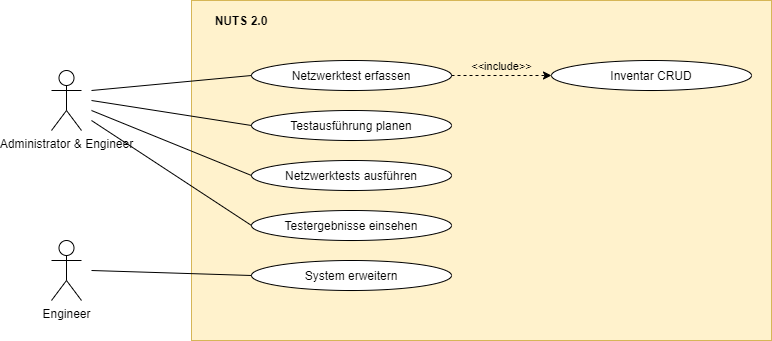
\includegraphics[scale=0.6]{\vorlagenOrdner/Bilder/UseCaseDiagram}
		\end{center}
		\caption{Use Case Diagramm}
	\end{figure}
		
\section{Nichtfunktionale Anforderungen}
	In diesem Kapitel werden die nichtfunktionalen Anforderungen an das Projekt behandelt.
	Es werden Aspekte und Anforderungen aus den Bereichen Änderbarkeit, Benutzbarkeit, Effizienz, Zuverlässigkeit, Betreibbarkeit und Sicherheit betrachtet.
	Die jeweiligen Aspekte werden in ihren Unterkapiteln genauer beschrieben.
	Es werden mögliche Szenarien beschrieben, die in der Erstellung oder dem Betrieb der Software auftreten können und bei der Architektur in betracht gezogen werden.

	\subsection{Änderbarkeit}
		Aufwand, der zur Durchführung von vorgegebenen Änderungsarbeiten benötigt wird.
		Unter Änderungen gehen Korrekturen, Anpassungen oder Veränderungen der Umgebung, Anforderungen oder funktionalen Spezifikation.
		Gemäss ISO 9126 gehören zur Änderbarkeit folgende Teilmerkmale:
		
		\subsubsection{Analysierbarkeit}
			Aufwand, der benötigt wird, um das System zu verstehen, z.B. um Ursachen von Versagen oder Mängel zu diagnostizieren oder Änderungen zu planen.

		\subsubsection{Modifizierbarkeit}
			Wie leicht lässt sich das System anpassen, um Verbesserungen oder Fehlerbeseitigungen durchzuführen.

		\subsubsection{Stabilität}
			Wahrscheinlichkeit, dass mit Änderungen unerwartete Nebenwirkungen auftreten.

		\subsubsection{Testbarkeit}
			Wie gross wird der Aufwand, bei Änderungen die Software zu prüfen.

		\newpage

		\subsubsection{Szenario: Neue Netzwerkschnittstelle}
			Wenn zum bestehenden System eine neue Netzwerkschnittstelle definiert werden soll, so muss die dafür notwendige Software innerhalb von einer Arbeitswoche entwickelt, integriert und in Betrieg genommen werden können.
			
			\begin{table}[!h]
				\begin{tabularx}{\textwidth}{lX}
					\toprule
					Qualitätsziele & Flexibilität, Erweiterbarkeit, Anpassbarkeit, Austauschbarkeit  \\
					\midrule
					Geschäftsziel(e) & Software kann mit geringem Aufwand an geänderte Anforderungen angepasst werden  \\
					\midrule
					Auslöser & Ein Engineer möchte weitere Tests einbinden oder Schnittstellen, die nicht im System integriert sind.  \\
					\midrule
					Reaktion & Die Software lässt sich von einem Entwickler in weniger als einer Woche um benötigte Komponenten erweitern.  \\
					\midrule
					Zielwert & 	Erweiterungen der Netzwerkschnittstellen oder Anpassungen von Tests sind innerhalb von 40 Personenstunden umsetzbar.  \\
					\bottomrule
				\end{tabularx}
				\caption{Szenario: Neue Schnittstelle}
			\end{table}
			

		\subsection{Scenario: Schnelle Fehlerlokalisierung}
			Die Ursache von fehlgeschlagenen Tests (Software-Unittests) lässt sich in kurzer Zeit lokalisieren.
			
			\begin{table}[!h]
				\begin{tabularx}{\textwidth}{lX}
					\toprule
					Qualitätsziele & Schnelle Fehlerbehebung, Änderbarkeit, Anpassbarkeit, geringes Risiko bei Erweiterungen  \\
					\midrule
					Geschäftsziel(e) & Entwickler können das Programm einfach anpassen und erkennen im Fehlerfall schnell, was nicht funktioniert hat.  \\
					\midrule
					Auslöser & Eine Änderung im Code führt zu Fehlnern in der Ausführung.  \\
					\midrule
					Reaktion & Wenn ein Fehler dazu führt, dass die Softwareausführung fehlschlägt, kann ein Entwickler aufgrund von Fehler- und/oder Log-Nachrichten die Ursache in kurzer Zeit lokalisieren.  \\
					\midrule
					Zielwert & Fehlerlokalisierung findet durchschnittlich in weniger als 10 Minuten statt.  \\
					\bottomrule
				\end{tabularx}
				\caption{Szenario: Schnelle Fehlerlokalisierung}
			\end{table}
			
			\newpage

	\subsection{Benutzbarkeit}
		Zeitlicher Aufwand, der für die Erlernung der Benutzung des Programms benötigt wird. 
		Die User werden hierfür in spezifische Nutzergruppen mit festgelegten Fähigkeiten unterteilt.
		
		\subsubsection{Verständlichkeit}
			Aufwand für den Nutzer, die Konzepte und Menüführung der Anwendung zu verstehen.

		\subsubsection{Erlernbarkeit}
			Aufwand für den User, sich ohne Vorwissen in das System einzuarbeiten.

		\subsubsection{Bedienbarkeit}
			Aufwand für den Benutzer, die Anwendung zu bedienen.

		\subsubsection{Szenario: Einfachheit der Definitionssprache}
			Die Definitionen von Inventar und Tests sind so aufgebaut, dass ein User in kurzer Zeit die Struktur und den Aufbau versteht und eigene Tests implementieren kann.
			
			\begin{table}[!h]
				\begin{tabularx}{\textwidth}{lX}
					\toprule
					Qualitätsziele & Produktivität, Einfachheit, Verständlichkeit \\
					\midrule
					Geschäftsziel(e) & Einarbeitung in die Testdefinition erfolg möglichst einfach und benötigt nur geringes Vorwissen.  \\
					\midrule
					Auslöser & Ein Nutzer, welcher keine Erfahrung im Umgang mit der Software hat, möchte eigene Tests definieren.  \\
					\midrule
					Reaktion & Benutzer können sich schnell in die Testdefinitionen einlesen und rasch eigene Tests definieren, vorausgesetzt, sie haben Kenntnisse des Netzwerkes.  \\
					\midrule
					Zielwert & Ungeschulte Nutzer verstehen innerhalb von durchschnittlich 30 Minuten die Struktur und den Aufbau der Testdefinitionen und sind in der Lage, eigene Tests zu erstellen.  \\
					\bottomrule
				\end{tabularx}
				\caption{Szenario: Einfachheit der Definitionssprache}
			\end{table}
			\newpage
			
		\subsubsection{Szenario: Hinweis auf Fehleingaben}
		Fehlerhafte Eingaben werden vom System ignoriert und der Benutzer wird auf die falsche Eingabe hingewiesen. Das Programm führt fehlerfreie Programmteile unabhängig von den Fehlern durch.
		
		\begin{table}[!h]
			\begin{tabularx}{\textwidth}{lX}
				\toprule
				Qualitätsziele & Robustheit, Verständlichkeit, Fehlertoleranz.  \\
				\midrule
				Geschäftsziel(e) & Fehleingaben führen nicht dazu, dass die Tests nicht mehr durchgeführt werden können.  \\
				\midrule
				Auslöser & Ein Benutzer macht einen Fehler bei der Testdefinition und startet das Programm.  \\
				\midrule
				Reaktion & Das Programm führt alle korrekten Tests durch und informiert den Benutzer, dass es fehlerhafte Tests gibt, die nicht durchgeführt werden können. Die Hinweise werden im Report und auf der Konsolenausgabe geschrieben.   \\
				\midrule
				Zielwert & Tests sind einzeln gekapselt und werden unabhängig voneinander durchgeführt. Falscheingaben werden vom Programm detektiert und im Testreport sowie auf der Konsolenausgabe erwähnt.  \\
				\bottomrule
			\end{tabularx}
			\caption{Szenario: Hinweis auf Fehleingaben}
		\end{table}
		
		
	\subsection{Effizienz}
	Mit Effizienz ist die 'performance efficiency' gemeint, d.h. das Verhältnis zwischen dem Leistungsniveau der Software und den eingesetzten Hardwarekomponenten. 
	Andere Beschreibungen umfassen: Skalierbarkeit, Speicherbedarf, Verarbeitungsgeschwindigkeit, Antwortzeit etc.
	Teilmerkmale nach ISO 9126:

		\subsubsection{Zeitverhalten}
		Dauer für Verarbeitung und Antwortzeit sowie Durchsatz bei der Ausführung des Programms

		\subsubsection{Verbrauchsverhalten}
		Wie viel Speicherbedarf hat das Programm, wie lange werden Betriebsmittel in Anspruch genommen und welche Hardwarekomponenten werden benötigt.

	\subsection{Zuverlässigkeit}
	Unter Zuverlässigkeit versteht man die Fähigkeit der Software, unter festgelegten Bedingungen die Funktionalität über einen definierten Zeitraum zu gewährleisten
	
		\subsubsection{Reife}
		Geringe Ausfallhäufigkeit durch Fehlzustände.

		\subsubsection{Fehlertoleranz}
		Die Software ist in der Lage, trotz Fehlern ihr spezifiziertes Leistungsniveau beizubehalten.

		\subsubsection{Wiederherstellbarkeit}
		Im Fehlerfall können betroffene Daten wiederhergestellt und die Funktionalität wieder aufgenommen werden.

		\subsubsection{Szenario: Tests lassen sich auf der Netzwerkseite nicht ausführen}
		Falls ein Test auf dem jeweiligen Netzwerkgerät nicht erfolgreich durchgeführt werden kann, läuft das Programm weiter und definiert den dazugehörigen Netzwerktest als nicht bestanden.
		
		\begin{table}[!h]
			\begin{tabularx}{\textwidth}{lX}
				\toprule
				Qualitätsziele & Robustheit, Behandlung Infrastrukturbedingter Fehler.  \\
				\midrule
				Geschäftsziel(e) & Das System führt alle Tests unabhängig voneinander durch. Wenn ein Test zu einem Fehler führt, weil z.B. ein falsches Netzwerkgerät angegeben wurde, wird dieser Test unabhängig von allen anderen Tests fehlschlagen.  \\
				\midrule
				Auslöser & Test lässt sich auf spezifizierter Infrastruktur nicht ausführen.  \\
				\midrule
				Reaktion & Test schlägt fehl und mögliche Ursachen werden im Report und in der Konsole angezeigt. Alle anderen Tests laufen durch.  \\
				\midrule
				Zielwert & Das Fehlschlagen eines Tests fürht nicht zum Programmabbruch.  \\
				\bottomrule
			\end{tabularx}
			\caption{Szenario: Testausführung Netzwerkseitig nicht ausführbar}
		\end{table}
		

	\subsection{Betreibbarkeit}
	Die Betriebbarkeit wird in der ISO 9126 nicht definiert. Die ISO spezifiziert aber mehrere Teilmerkmale, die unter dem Begriff Betreibbarkeit zusammengefasst werden können:

		\subsubsection{Analysierbarkeit}
		Aufwand, der benötigt wird, um den Code zu analysieren, um im falle eines Versagens dessen Ursachen zu diagnostizieren oder um Änderungen zu planen und durchzuführen.

		\subsubsection{Installierbarkeit}
		Aufwand, das Programm auf einem frisch aufgesetzten Gerät laufen zu lassen.

		\subsubsection{Übertragbarkeit}
		Kann die Software von einer Umgebung auf eine andere übertragen werden. 
		Als Umgebung zählen Hardwarekomponenten, Softwarekomponenten, Organisatorische Umgebungen oder Betriebssysteme. 

		\subsubsection{Austauschbarkeit}
		Aufwand und Möglichkeit, die Software anstelle einer anderen in deren spezifizierten Umgebung laufen zu lassen.

		\subsubsection{Koexistenz}
		Fähigkeit der Software, neben anderen Programmen mit ähnlichen oder übereinstimmenden Funktionen zu arbeiten.

		\subsubsection{Szenario: Einfache Installation auf einem neuen Gerät}
		Das Programm lässt sich auf einem neuen Gerät ohne grossen Mehraufwand installieren, ohne dass die Funktionalität des Geräts beeinflusst wird.
		
		\begin{table}[!h]
			\begin{tabularx}{\textwidth}{lX}
				\toprule
				Qualitätsziele & Einfachheit, Portierbarkeit, Benutzbarkeit  \\
				\midrule
				Geschäftsziel(e) & Die Installation der Software ist so einfach, dass sie innert kurzer Zeit und/oder automatisiert durchgeführt werden kann.  \\
				\midrule
				Auslöser & Die Testsoftware soll auf einem frisch aufgesetzten Gerät installiert werden.  \\
				\midrule
				Reaktion & Installationszeiten sind gering, benötigen wenige bis keine weiteren Softwarekomponenten oder lässt sich mit einigen Kommandozeilenbefehlen automatisch installieren.  \\
				\midrule
				Zielwert & Die Software wird mit einer Installationsanleitung ausgeliefert, die einfach und verständlich die Inbetriebnahme des Programms erklärt. Abhängigkeiten zu anderen Softwarekomponenten werden bewusst gering gehalten um eine einfache Installation mit weniger als 30 Minuten Zeitaufwand zu gewährleisten.  \\
				\bottomrule
			\end{tabularx}
			\caption{Szenario: Einfache Installation auf einem anderen Gerät}
		\end{table}
		


	\subsection{Sicherheit}
	In dieser Sektion werden Sicherheitsanforderungen beschrieben. 
	Verschlüsselung, Privacy und der Umgang mit Passwörtern.

		\subsubsection{Verschlüsselung von Datenübertragungen}
		Die Netzwerktest werden über eine Verschlüsselte Verbindung durchgeführt, die dem aktuellen Stand der Technik entspricht.

		\subsubsection{Umgang mit Passwörtern}
		Zugangsdaten der Devices werden im Inventar in Unverschlüsselter Form abgelegt. Es liegt in der Verantortung der Betreiber des Netzwerks, dass die Zugangsdaten nicht von dritten eingesehen werden.
\end{document}